\section{SIMD-nodes}

All SIMD nodes shares the same instruction set and execute instructions in
parlell. {\tt Word} size is 8 bit. Each SIMD node is fully equipped with
registers, aritmetic logic unit (ALU), message passing and instruction handling
through the SIMD Node instruction set detailed in this page.

The schematic of a SIMD node is shown in figure
\ref{fig:fpga-simd-arch}. \TODO{Talk around the figure}

\begin{figure}[h]
  \centering
 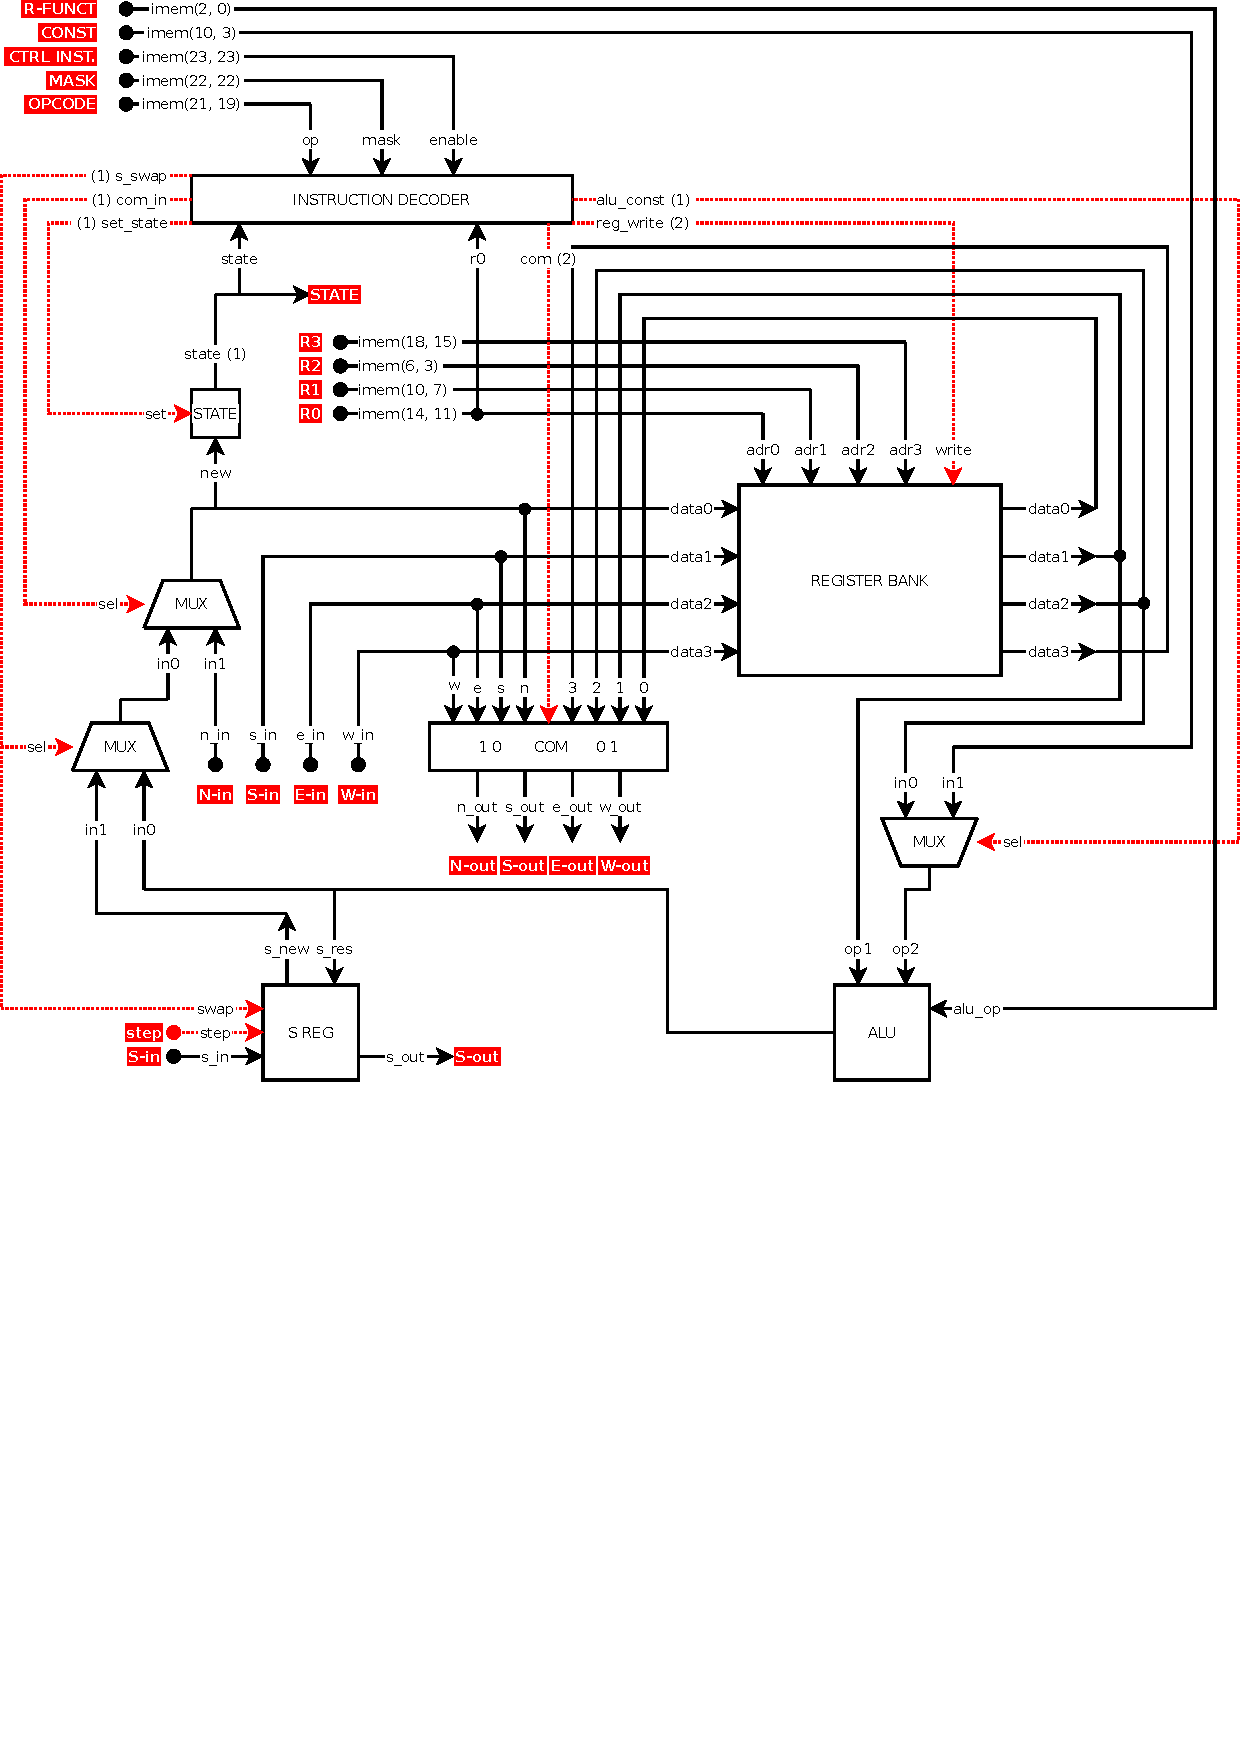
\includegraphics[width=\linewidth,clip,trim=0 0 0 0]
                  {fig/fpga/fpga-simd-arch.pdf}
  \caption{LENA SIMD architecture}
  \label{fig:fpga-simd-arch}
\end{figure}


\subsection{Components}
In order to the keep the signals to a minimum, the simd node is nicely divieded
into seperate components which makes up the datapath for the node.

\subsection{Instruction Decoder}
This is the node's control component. It takes the OP-code of the instruction
and sets control signals for all the other components in the node.

\subsection{I/O Controller}

\subsection{Register Bank}

\subsection{ALU}

\subsection{S Register}
The S REG (source data register) is a special purpose register within the SIMD
node and holds the next source data for the node. It is partly controlled by the
node's instruction set and partly controlleb by a special {\tt step} signal form
the DMA.

This register also has the capability to recieve data from the left node,
through the {\tt s\_in}-bus, and passing it along to node on the right through
the {\tt s\_out}-bus when instructed by the {\tt step} singal. This allows a
suimultanious data transfer while the node is busy processing.

Rising the value on the {\tt swap} control signal will write the result from the
ALU to the S\_REG and compy the data from the S\_REG out to the {\tt s\_new}
bus, ultimatly writing this data to the register bank.

\subsection{State Register}

\subsection{Registers}
Each SIMD node have $2^4$ general purpose registers. 4 of these are avaiable for
general storage when executing instructions. The remaining 2 registers are the
special purpose registers {\tt \$zero} and {\tt \$state}.

\begin{table}[h]
  \centering
  \begin{tabularx}{\linewidth}{XXXXXXXXX}\toprule
    R0 & R1 & R2 & R3 & R4 & R5 & R6 & R7 \\ \midrule
    \tt \$zero & \tt \$r1 & \tt \$r2 & \tt \$r3 & \tt \$r4 & \tt \$r5 &
    \tt \$r6 & \tt \$r7\\ \bottomrule
  \end{tabularx}
  \begin{tabularx}{\linewidth}{XXXXXXXX}
    R8 & R9 & R10 & R11 & R12 & R13 & R14 & R15 \\ \midrule
    \tt \$r8 & \tt \$r9 & \tt \$r10 & \tt \$r11 & \tt \$r12 & \tt \$r13 &
    \tt \$r14 & \tt \$state\\ \bottomrule
  \end{tabularx}
  \caption{Registers in the SIMD nodes}
  \label{tab:simd-registers}
\end{table}


\subsection{State-register}

\subsection{Zero-register}

\subsection{BRAM and SRAM}
Block RAM (BRAM) or Static RAM (SRAM) are not available form the SIMD node.

\subsection{Instruction Set}
SIMD nodes operates on an {\tt 24 bit} instruction set divided into 2 main
formats. Arithmetic instructions (R, I and S) and message passing instructions
(M-send, M-store and M-forward).

\subsection{Ideology}

\subsection{R-Format (OP = 000)}
Arithmetic register functions instructions

\begin{table}[h]
  \centering
  \begin{tabular}{cccccccc}\toprule
    \thx{ctrl} & \thx{mask} & \thx{op} & \thx{rs} & \thx{rt} & \thx{rd} &
    \thx{n/a} & \thx{fn} \\ \midrule
    1 bit & 1 bit & 3 bit & 4 bit & 4 bit & 4 bit & 4 bit & 3 bit
    \\ \bottomrule
  \end{tabular}
  \caption{Arithmetic register function instructions}
  \label{tab:ar-re-fu-in}
\end{table}


\begin{itemize}
\item {\tt ctrl} must be set to 0 in order to be executed on the SIMD node.
\item {\tt mask} is set to 1 for selectively enabling the node when executing
  conditional branches.
\item {\tt op} this is the instruction op-code.
\item {\tt rs} write data register address.
\item {\tt rt} read data 1 register address.
\item {\tt rd} read data 2 register address.
\item {\tt n/a} not assigned for R-instructions.
\item {\tt fn} is the artimetic operation to perform.
\end{itemize}

\begin{table}[h]\small
  \centering
  \begin{tabularx}{1.03\textwidth}{lccX}\toprule
    \thx{name} & \thx{fn} & \thx{assembly code} & \thx{binary representation}
    \\ \midrule
    \thx{add} & \tt 000 & \tt add \$rs, \$rt, \$rd &
    \tt 0 m 000 ssss tttt dddd ---- 000\\
    \thx{sub} & \tt 001 & \tt sub \$rs, \$rt, \$rd &
    \tt 0 m 000 ssss tttt dddd ---- 001\\
    \thx{slt} & \tt 010 & \tt slt \$rs, \$rt, \$rd &
    \tt 0 m 000 ssss tttt dddd ---- 010\\
    \thx{and} & \tt 011 & \tt and \$rs, \$rt, \$rd &
    \tt 0 m 000 ssss tttt dddd ---- 011\\
    \thx{or}  & \tt 100 & \tt or~ \$rs, \$rt, \$rd &
    \tt 0 m 000 ssss tttt dddd ---- 100\\
    \thx{eq}  & \tt 101 & \tt eq~ \$rs, \$rt, \$rd &
    \tt 0 m 000 ssss tttt dddd ---- 101\\
    \thx{sll} & \tt 110 & \tt sll \$rs, \$rt, \$rd &
    \tt 0 m 000 ssss tttt ---- ---- 110\\
    \thx{srl} & \tt 111 & \tt srl \$rs, \$rt, \$rd &
    \tt 0 m 000 ssss tttt ---- ---- 111\\ \bottomrule
  \end{tabularx}
  \caption{List of R-instructions}
  \label{tab:r-instructions}
\end{table}


\subsection{I-Format (OP = 001)}
Immediate functions using constants.

\begin{table}[h]
  \centering
  \begin{tabular}{ccccccc}\toprule
    \thx{ctrl} & \thx{mask} & \thx{op} & \thx{rs} & \thx{rt} & \thx{const} &
    \thx{fn} \\ \midrule
    1 bit & 1 bit & 3 bit & 4 bit & 4 bit & 8 bit & 3 bit
    \\ \bottomrule
  \end{tabular}
  \caption{Immediate functions using constants}
  \label{tab:immediate-fn-const}
\end{table}


\begin{itemize}
\item {\tt ctrl} must be set to 0 in order to be executed on the SIMD node.
\item {\tt mask} is set to 1 for selectivly enabling the node when executing
  conditional branches.
\item {\tt op} this is the instruction op-code.
\item {\tt rs} write data register address.
\item {\tt rt} read data 1 register address.
\item {\tt const} constant value (immediate).
\item {\tt fn} is the artimetic operation to perform.
\end{itemize}

\TODO{Is the font size ok?}
\begin{table}[h]\small
  \centering
  \begin{tabularx}{1.03\linewidth}{lccX}\toprule
    \thx{name} & \thx{fn} & \thx{assembly code} & \thx{binary representation}
    \\ \midrule
    \thx{add} & \tt 000 & \tt addi \$rs, \$rt, \$rd &
    \tt 0 m 001 ssss tttt cccccccc 000\\
    \thx{sub} & \tt 001 & \tt subi \$rs, \$rt, \$rd &
    \tt 0 m 001 ssss tttt cccccccc 001\\
    \thx{slt} & \tt 010 & \tt slti \$rs, \$rt, \$rd &
    \tt 0 m 001 ssss tttt cccccccc 010\\
    \thx{and} & \tt 011 & \tt andi \$rs, \$rt, \$rd &
    \tt 0 m 001 ssss tttt cccccccc 011\\
    \thx{or}  & \tt 100 & \tt ori~ \$rs, \$rt, \$rd &
    \tt 0 m 001 ssss tttt cccccccc 100\\
    \thx{eq}  & \tt 101 & \tt eqi~ \$rs, \$rt, \$rd &
    \tt 0 m 001 ssss tttt cccccccc 101\\
    \thx{sll} & \tt 110 & \tt slli \$rs, \$rt, \$rd &
    \tt 0 m 001 ssss tttt -------- 110\\
    \thx{srl} & \tt 111 & \tt srli \$rs, \$rt, \$rd &
    \tt 0 m 001 ssss tttt -------- 111\\ \bottomrule
  \end{tabularx}
  \caption{List of I-instructions}
  \label{tab:i-instructions}
\end{table}


\subsection{S-Format (OP = 010)}
Swap source data register with processed data and store new source data in
register.

\begin{table}[h]
  \centering
  \begin{tabular}{cccccccc}\toprule
    \thx{ctrl} & \thx{mask} & \thx{op} & \thx{rs} & \thx{rt} & \thx{rd} &
    \thx{n/a} & \thx{fn} \\ \midrule
    1 bit & 1 bit & 3 bit & 4 bit & 4 bit & 4 bit & 4 bit & 3 bit \\ \bottomrule
  \end{tabular}
  \caption{S-format instructions}
  \label{tab:s-fmt-instr}
\end{table}


\begin{itemize}
\item {\tt ctrl}  must be set to 0 in order to be executed on the SIMD node.
\item {\tt mask} is set to 1 for selectivly enabling the node when executing
  conditional branches.
\item {\tt op}   this is the instruction op-code.
\item {\tt rs}   new source data register address.
\item {\tt rt}   old source data register adddress.
\item {\tt rd}   must be 000000.
\item {\tt n/a}  not assigned for S-instructions.
\item {\tt fn}   must be 000.
\end{itemize}

\begin{table}[h]\small
  \centering
  \begin{tabularx}{\textwidth}{lccX}\toprule
    \thx{name} & \thx{fn} & \thx{assembly code} & \thx{binary representation}
    \\ \midrule
    \thx{swap} & \tt 000 & \tt swap \$rs, \$rt &
    \tt 0 m 001 ssss tttt 0000 ---- 111\\ \bottomrule
  \end{tabularx}
  \caption{List of S instructions}
  \label{tab:s-instructions}
\end{table}



\subsection{M-Format (OP = 100, 101, 110)}
Send, recieve and forward data from and to neighbour nodes in all directions (north, south, east and west).

\begin{table}[h]
  \centering
  \begin{tabular}{cccccccc}\toprule
    \thx{ctrl} & \thx{mask} & \thx{op} & \thx{n} & \thx{s} & \thx{e} &
    \thx{w} & \thx{n/a} \\ \midrule
    1 bit & 1 bit & 3 bit & 4 bit & 4 bit & 4 bit & 4 bit & 3 bit \\ \bottomrule
  \end{tabular}
  \caption{M format instructions}
  \label{tab:m-fmt-instr}
\end{table}


\begin{itemize}
\item {\tt ctrl} must be set to 0 in order to be executed on the SIMD node.
\item {\tt mask} is set to 1 for selectivly enabling the node when executing
  conditional branches.
\item {\tt op} this is the instruction op-code.
\item {\tt n} north data write or read register address.
\item {\tt s} south data write or read register address.
\item {\tt e} east data write or read register address.
\item {\tt w} west data write or read register address.
\item {\tt n/a} no ALU operations applicable.
\end{itemize}

\begin{table}[h]
  \begin{tabularx}{\textwidth}{lrcc}\toprule
    \thx{name} & \thx{OP} & \thx{assembly code}
    \\ \midrule
    \thx{send} & \tt 100 & \tt send~ \$r1, \$r2, \$r3, \$r4\\
    \thx{store} & \tt 101 & \tt store \$r1, \$r2, \$r3, \$r4\\
    \thx{store \& forward} & \tt 110 & \tt frwrd \$r1, \$r2, \$r3, \$r4
    \\ \bottomrule
  \end{tabularx}
  \begin{tabularx}{\textwidth}{lX}
    \thx{name} & \thx{binary representation} \\ \midrule
    \thx{send} & 
    \tt 0 m 100 nnnn ssss eeee wwww ---\\
    \thx{store} &
    \tt 0 m 101 nnnn ssss eeee wwww ---\\
    \thx{store \& forward} & 
    \tt 0 m 110 nnnn ssss eeee wwww ---\\ \bottomrule
  \end{tabularx}    
  \caption{List of M-instructions}
  \label{tab:m-instructions}
\end{table}


In figure \ref{tab:m-instructions} we see the different \ldots.  \thx{store \&
  forward} forwards according to the 4-way data exchange patterns (N
$\rightarrow$ E, E $\rightarrow$ S, S $\rightarrow$ W, W $\rightarrow$ N).

{\tt PRO TIP} \TODO{Better avoid calling it PRO TIP in the report}
M-instruction, especially send and forwards, must be issued with mask bit set to
0 in order to get data from all the nodes and not only those withich are
execuriting withing a conditional branch (status = 1).

\begin{figure}[h]
  \centering
  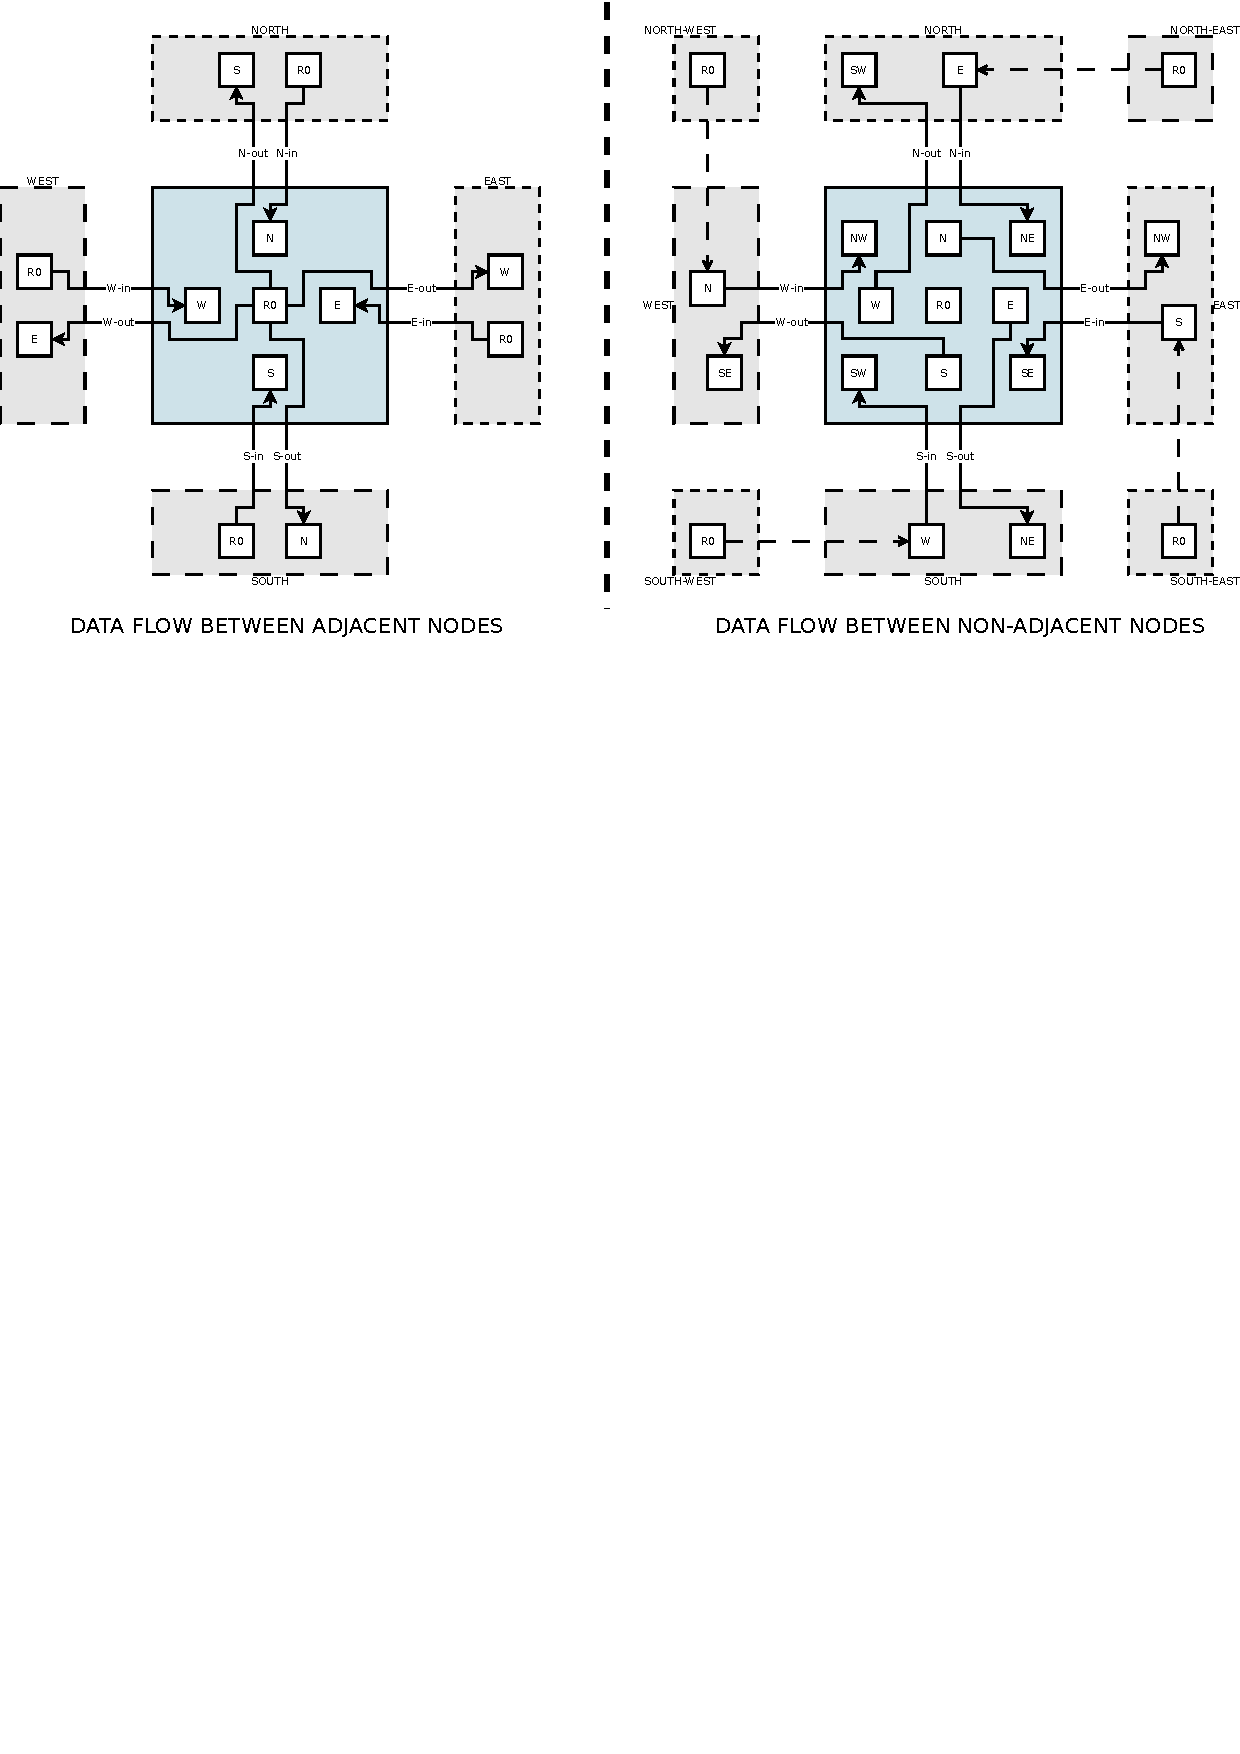
\includegraphics[width=\linewidth,clip,trim=0 18cm 0 0]
                  {fig/fpga/fpga-simd-datacom.pdf}
  \caption{Four-way communication in the LENA SIMD array.}
  \label{fig:fpga-simd-datacom}
\end{figure}
\TODO{Split up into 3 figures instead?}


\subsection{Branching}
Since all nodes run the same instructions, both parts of a branch must be
executed. Nodes are setting the {\tt state} to 1 in order to indicate that they
are executing within that part of the branch.

\begin{table}[h]
  \centering
  \begin{tabularx}{\textwidth}{rlcX}\toprule
    \thxc{step} & \thxc{instruction} & \thxc{state} & \thxc{description} \\
    \midrule
    0 & \tt // initial state & 0 & \\
    1 & \tt eq \$state \$r1, \$r2 & 1
    & Set state to 1 if branch should be taken for the node.\\
    \ldots & \tt // branch taken & 1 &
    Instructions for when the branch is taken.\\
    2 & \tt eq \$state, \$state, \$zero & 0 & Negate the state.\\
    \ldots & \tt // branch not taken & 0 & Instructions for when the branch is
    not taken.\\ \bottomrule
  \end{tabularx}
  \caption{Single level branching}
  \label{tab:single-level-branching}
\end{table}


\subsection{Multi-level branching}
Since state register is 8 it is possible to have up-to 8 nested branches by
shifting the current state to the left and adding the new state to the
end. Below \TODO{Refer to table, not relative to where it is placed} are the
instructions for performing a multilevel-branch.

\CHECK{Better switch out zeroes and ones with x'es and y's?}
\begin{table}[h] % TODO: Drag out
  \centering
  \begin{tabularx}{\textwidth}{rlcX}\toprule
    \thxc{step} & \thxc{instruction} & \thxc{state} & \thxc{description} \\
    \midrule
    0 & \tt // initial state & 01 & \\
    1 & \tt sll \$r3, \$state & 01
    & Save the current state by shifting left.\\
    2 & \tt eq \$r4 \$r1, \$r2 & 01
    & Calculate if branch is taken for the node.\\
    3 & \tt add \$state \$r4, \$r3 & 11
    & Set the new state.\\
    \ldots & \tt // branch taken & 11 &
    Instructions for when the branch is taken.\\
    4 & \tt andi \$r3, \$state, 1111 1110 & 11
    & Save the old state for the node.\\
    5 & \tt andi \$r4, \$state, 0000 0001 & 11 & Save the current state.\\
    6 & \tt eq \$r4, \$r4, \$zero & 11 & Negate the current state.\\
    7 & \tt add \$state, \$r4, \$r3 & 10 & Set new state.\\
    \ldots & \tt // branch not taken & 10
    & Instructions for when the branch is not taken.\\
    8 & \tt srl \$state, \$state & 01 & Revert to state before branch by
    shifting right.\\ \bottomrule
  \end{tabularx}
  \caption{Multi level branching}
  \label{tab:multi-level-branching}
\end{table}

\CHECK{Could any of these tables be figures instead?}
